% Name: Flow network
% Description: A maximum flow of value 23 from s to t, with each edge labeled flow over capacity and the saturated edges in orange.
% Tags: flow network, maximum flow, capacity, Ford-Fulkerson

\usetikzlibrary{arrows.meta}

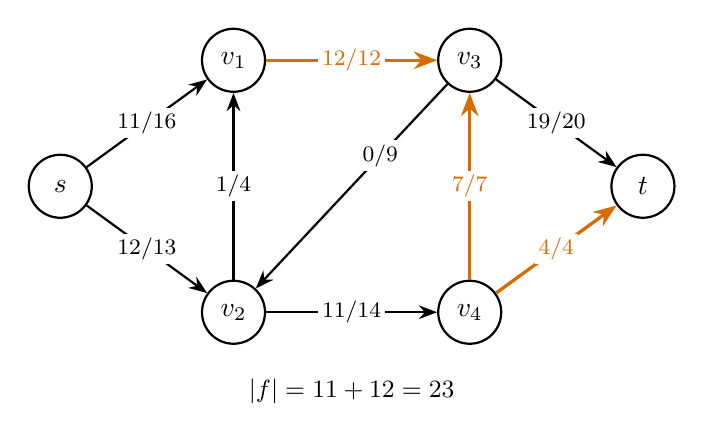
\begin{tikzpicture}[
  >={Stealth}, every edge/.style={draw, ->, thick},
  vertex/.style={circle, draw, thick, minimum size=8mm, inner sep=0pt},
  full/.style={orange!85!black, very thick},
  amount/.style={font=\footnotesize, fill=white, inner sep=1.5pt},
]
  \node[vertex] (s) at (0,0) {$s$};
  \node[vertex] (v1) at (2.2,1.6) {$v_1$};
  \node[vertex] (v2) at (2.2,-1.6) {$v_2$};
  \node[vertex] (v3) at (5.2,1.6) {$v_3$};
  \node[vertex] (v4) at (5.2,-1.6) {$v_4$};
  \node[vertex] (t) at (7.4,0) {$t$};
  % Conservation: v1 12 in and out, v2 12, v3 19, and v4 11.
  \path (s) edge node[amount] {11/16} (v1)
        (s) edge node[amount] {12/13} (v2)
        (v2) edge node[amount] {1/4} (v1)
        (v1) edge[full] node[amount] {12/12} (v3)
        (v3) edge node[amount, pos=0.35] {0/9} (v2)
        (v2) edge node[amount] {11/14} (v4)
        (v4) edge[full] node[amount] {7/7} (v3)
        (v3) edge node[amount] {19/20} (t)
        (v4) edge[full] node[amount] {4/4} (t);
  \node[font=\small] at (3.7,-2.6) {$|f| = 11 + 12 = 23$};
\end{tikzpicture}
